\section{Related Work}

\subsection{\cite{LabelingLanguageLearning}: In-Situ Labeling for Augmented Reality Language Learning}
%Huynh-2019 In-Situ Labeling for Augmented Reality Language Learning.
\cite{LabelingLanguageLearning} schafft ein Framework, mit dem die Lernmethode "loci" in Augmented Reality umgesetzt und erweitert werden kann. Die Lernmethode beruht darauf, Gegenstände der Welt mit Notizen zu beschriftet. 

Dafür wurde folgende automatische real-time Objekt Erkennung entwickelt:

Mithilfe von Image Based Object Detection werden Objekte auf Fotos der AR Umgebung erkannt. Diese Objekte werden dann in die 3D Szene der Umgebung übernommen. 

Die AR Brille hat zu wenig Rechenleistung, um Image Based Object Detection durchzuführen. Daher wurde eine Server Client Architektur aufgesetzt.

Die Videokamera der AR Brille wird verwendet um Bilder von der Umgebung aufzunehmen. Die einzelnen Frames werden an den Server geschickt. Dieser nutzt ein Object Recognition Learning Modell um alle erkennbaren Objekte in dem Bild zu finden und mit Bounding Boxen zu lokalisieren.

Die ObjectDetection API von TesnorFlow wird verwendet. Es findet mehere Objekte in einem Foto in einer Analyse und gibt Bounding Boxen an. Damit die Objekt Erkennung in real-time durchgeführt werden kann, wird die niedrigeste Kamera Auflösung mit 896x504 verwendet. Zusätzlich werden die Fotos als JPEG mit 50 Prozent Qualität komprimiert. Damit braucht die Analyse 30 ms pro Foto, was eine Real-Time Erkennung mit 30 frames per second erlaubt. 

Trotzdem ist die Erkennung in der Applikation verspätet, durch einen Netzwerk Delay von 150ms zwischen der Hololens und dem Server, der die Foto-Analyse durchführt.

Die Hololens nummeriert die Frames, die an den Server versicht werden. Zusätzlich wird für jedes der Frames, die Kameraposition gespeichert, mit der es aufgenommen wurde. So können Frames asynchrom analysiert werden. 

Ist die Analyse durchgelaufen, wird die Bounding Boxen der Objekte und die Kameraposition genutzt, um die Objekte in der 3D Umgebung zu lokalisieren. Dafür wird der Mittelpunkt jeder Bounding Box mithilfe eines Raycastes in die 3D Szene projiziert.

Um Fehlern bei der Object Erkennung entgegenzuwirken, wird ein Objekt erst als endgültig erkannt angesehen, wenn es auf meheren Fotos erkannt erkannt wurde. Mehrere Frames werden verwendet um die Position des Objekte abzuschätzen. Dann werden bereits existierende Label untersucht, die in den letzten 60 Frames aufgenommen wurden. Wenn die Labels nah beieinander liegen wird davon ausgegangen, das es sich um dasselbe Objekt handelt. Der Mittelpunkt der Labels wird zu der Position des Objektes und wird mit einem endgültigen Label versehen.

%wenn das Objekt detection Model gut ist, muss man nicht so viele Position und false positive dinger ausmerzen.
%nicht echt zeit machen. 

\subsection{View Management for Vitual and Augmented Reality}
%todo

\cite{viewmanagement3d} beschreibt View Management für interkative 3D Benutzeroberflächen. Als View Management wird das positionieren von Labels bezeichnet.
Die Labels können sich auf eine 2D Ebene beschränken, oder im 3D Raum liegen. Das Ziel des View Management für AR ist es die Lables so zu positionieren, das sie einander und relevante reale Objekte nicht verdecken. Gleichzeitig sollen die Label Gegenständen der Realen Welt  auf eine verständliche weise annotieren. Sie sollen beispielsweise nahe bei den Objekten liegen, zu denen sie gehören.

Die Applikation die in dieser Arbeit erstellt wurde, verfügt über Label im 3D Raum. Die Lesbarkeit der Label kann durch View Management verbessert werden, indem die Positionen der Labels über zeit verändert wird, wenn mehr Labels hinzukommen. Durch das hinzukommen von Labels werden auch Gegenstände der realen Welt markiert. Im Zuge des View Managements kann sichergestellt werden, das die Gegenstände nicht verdeckt werden. 

View Management geht jedoch über den Rahmen dieser Arbeit hinaus.\citep{viewmanagement3d}

%4] K. Been, E. Daiches, and C. Yap. Dynamic map labeling. IEEE Transactions on Visualization and Computer Graphics, 12(5):773–780, Sep. 2006. doi: 10.1109/TVCG.2006.136
%[5] B. Bell, S. Feiner, and T. H¨ollerer. View management for virtual and augmented reality. In Proceedings of the 14th Annual ACM Symposium on User Interface Software and Technology, UIST ’01, pp. 101–110.

\subsection{Context aware Mixed Reality}
%todo

\cite{contextawaremixedreality} stellen ein Framework vor, in dem einer AR Umgebung semantische Eigenschaften zugewiesen wird um realistische Interaktionen zwischen virtuellen und realen Objekten zu erreichen. 
Insbesondere sollen physikalische Interaktionen realistischer werden.

Das Framework reichert die Umgebung mit Informationen über die Materialien an, aus denen reale Oberflächen und Gegenstände bestehen. Die Materialien werden mit Labels versehen und die physikalischen Interaktionen berücksichtigen die Materialien der Umgebung.

Als beispielhafte Applikation wurde ein First-Person-Shooter vorgestellt, bei dem das aussehen von Einschusslöchern davon anhängt auf welches Material geschossen wurde.

Für die Erkennung der Materialien werden Frames der Hololens nach Materialien segmentiert. Diese Analyse ist nicht Echtzeit fähig, die Interaktionen können jedoch in Echtzeit ablaufen. 
Die semantischen Informationen werden abgespeichert um bei späteren Interaktionen abgerufen zu werden. Die Erkennung der Materialien ist nicht Echtzeit fähig, aber durch das speichern der Materialien im Raum können die Interaktionen in echt Echtzeit ablaufen. Die Semantischen Informationen müssen nicht zu jedem Frame bestimmt werden, sondern nur in Abständen erhoben werden. 

Um die Semantik der Umgebung zu erheben, werden RGB-Bilder von ihr aufgenommen und mit einem neuronales Netzwerk analysiert. Das neuronale Netz wurde von \cite{contextawaremixedreality} für den First-Person-Shooter trainiert. Es kann 23 unterschiedliche Materialien erkennen und segmentiert Bilder danach. Dabei wird für jedes Pixel ein Material angegeben.

Mithilfe der Camera Position des Frames werden die Material-Informationen auf das 3D Modell der Umgebung projiziert. 

Ein Kinect Sensor wird als Tiefenkamera verwendet. 

Porblem damit das es pixelweise ist. und sich overlappen kann. 


\newpage
\section{Grundlagen}
\subsection{Grundlagen zu Augmented Reality}
\subsubsection{Augmented Reality} %Einfürhung in AR

Augmented Reality vermischt die reale Welt mit digitalen (virtuellen) Elementen um dem Nutzer eine erweiterte Wahrnehmung zu ermöglichen. Es können 3D Objekte, 2D Overlays oder Audioelemente verwendet werden um eine reale Umgebung mit Informationen zu bereichern. 

Die Umgebung bezeichnet den Teil der realen Welt, der in Augmented Reality abgebildet und erweitert werden soll. Beispielweise ein Zimmer, in dem eine AR Anwendung ausgeführt wird.
Die AR Umgebung umfasst die reale Umgebung und die virtuellen Elemente.

Augmented Reality weist drei grundlegende Merkmale auf. 
\begin{itemize}
	\item Die Kombination der Realität mit dem Virtuellen. Besteht darin, das die Realität mit virtuellen Elementen überlagert wird.
	\item Die Interaktion mit virtuellen Elementen erfolgt in Echtzeit.
	\item Virtuelle Elemente haben einen festen räumlichen Platz in der AR Umgebung.
\end{itemize}

Die Merkmal unterstützen ein möglichst nahtloses verschmelzen der realen Welt mit den virtuellen Elementen.

Die Navigation in einer AR Umgebung funktioniert, indem der Nutzer sich durch physikalisch durch die reale Umgebung bewegt. Die reale Umgebung und die virtuellen Elemente stehen immer in dem gleichen räumlichen Verhältnis zueinander.

Da die reale Welt immer zu sehen ist, gibt sie eine Referenz und einen Kontext für die virtuellen Objekte an. 
Beispielsweise steht die Größe von virtuellen Objekten immer in Relation zu der realen Umgebung.\citep{GrundlagenAR}
%BookVirutalReality chapter 1

%müssen Informationen über die Umgebung erfasst werden. %Es ist wichtig zu bestimmen welche Objekte sich in der Umgebung befinden, die durch AR erweitert werden soll.

\subsection{AR System}

Ein AR System besteht aus Hardware und Software, die benötigt wird um die Wahrnehmung der realen Welt mit virtuellen Elementen zu erweitern.

Die Vermischung der realen Welt mit virtuellen Elementen muss angezeigt werden.

Die Interaktion des Nutzers mit virtuellen Elementen, und die Interaktion von virtuellen Elementen mit der realen Welt muss Simuliert werden.

Ein AR System ist in der Regel nicht an einen bestimmten Ort gebunden. Das System kann in unterschiedlichen Umgebungen eingesetzt werden, die unterschiedliche reale Gegenstände aufweisen. AR Applikationen müssen unterschiedliche Umgebungen unterstützen.\citep{GrundlagenAR}

%book Virutal reality chapter 1

\subsection{Spatial Mapping} 
Um virtuelle Objekte an eine Umgebung anzupassen und die Interaktion zwischen virtuellen Objekten und der realen Umgebung zu ermöglichen, benötigt ein AR System Informationen über die Geometrie der Umgebung.

Mit den Sensoren der AR Hardware werden Informationen gesammelt, die aussagen über die Geometrie der Umgebung geben. Beispielsweise haben AR Geräte eine Tiefenkamera, die die Entfernung messen kann. Die Daten der Sensoren werden gesammelt und in Relation zu der Bewegung des Gerätes gesetzt um die Umgebung zu Rekonstruieren. Dieser Vorgang nennt sich Spatial Mapping. 

Mit der Entstehenden Spatial Map können digitale Elemente mit der Umgebung interagieren, diese verdecken oder von ihr verdeckt werden.\citep{spatialMapping} 

%todo: bilder von spatial mapping in unity mit Hololens


\subsection{View Management}
Die virtuelle Information, die einen teil der realen Welt bereichern werden meistens als 3D Elemente angezigt. 
Die Information kann jedoch auch in 2D Elementen angezeigt werden, die sich auf eine 2D Ebene beschränkt. Insbesondere Labels, die reale Objekte erklären, können auf diese Art angezeigt werden.

Das Layout der 2D Elemente auf der Ebene wird durch View Management optimiert.
Idealerweise werden die Elemente so positioniert, das sie sich Gegenseitig nicht verdecken, relevante Bereiche der realen Welt nicht verdecken.
Zusätzlich sollen sie nah an den Gegenständen der Realen Welt bleiben, die sie annotieren. Siehe Abbildung \ref{viewManagement}.

\begin{figure}[H]
	\centering
	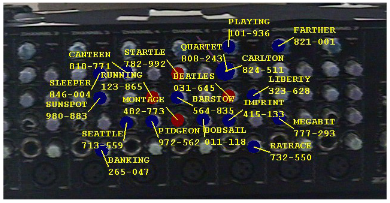
\includegraphics[width=0.7\textwidth]{images/ViewManagementImageFromPaper.PNG}
	\caption[]{Labels durch View Management positioniert.\citep{viewmanagement}}
	\label{viewManagement}
\end{figure}
Das Layout muss angepasst werden, wenn sich der View verändert. Gleichzeitig soll das Layout stabil bleiben und sich nicht verändern, wenn ein Anderes Layout ein wenig besser wäre, um ein hin und her springen zwischen zwei möglichen Layouts zu vermeiden.\citep{viewmanagement}

\subsection{Magic Leap AR Brille}

Die Magic Leap One Lightwear ist eine Augmented Reality Brille, die von dem Unternehmen Magic Leap entwickelt wurde. Sie verfügt über ein Head-Mounted Display und einer Recheneinheit die über ein Kabel mit dem Display verbunden ist. Die Recheneinheit kann an der Hüfte getragen werden, was die AR Brille komplett Mobil macht. 


\subsubsection{Hardware}

Die Recheneinheit besitzt zwei Denver 2.0 64 Bit Prozessor-Kerne und vier ARM Contex A57 46 bit Kerne. Davon ist einer der Denver Kerne und zwei der ARM Contex Kerne für Applikationen nutzbar.  

Sie besitzt neun Sensoren und mehrere Kameras. Dazu gehören:
\begin{itemize}
	\item ein Infrarot Tiefen-Sensor,
	\item ein Eye Tracker,
	\item eine Foto und Video Kamera, die im Format 16:9 mit einer Auflösung von 1920 x 1080 Pixeln aufnehmen,
	\item Umgebungskameras die in unterschiedliche Richtungen ausgerichtet sind. \citep{mlofficialsalespitch,mlglossary}
\end{itemize}

Der Output geschieht über ein Display mit einem 50 Grad Field of View und einem Seitenverhältnis von 4:3. Das Display ist transparent. Daher kann die reale Welt immer betrachtet werden. Selbst wenn ein weißes Objekt angezeigt wird, schimmert die reale Welt noch durch. 
Das Display kann keine Schwarzen Objekte anzeigen. 

Eingaben erfolgen über einen 6 Degree of Freedom Controller. Er verfügt über 3 Knöpfe (Trigger, Bumper, Home Button) und ein Touchpad. \citep{mlofficialsalespitch,mlglossary}

\begin{figure}[H]
	\centering
	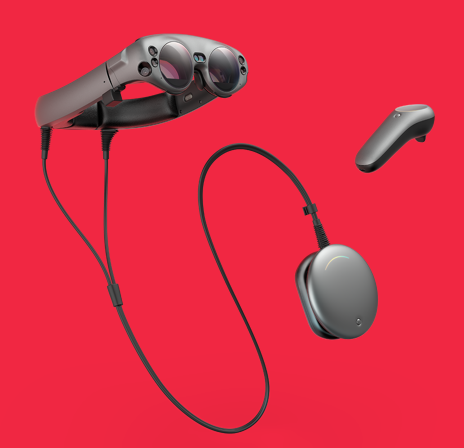
\includegraphics[width=0.7\textwidth]{images/img_magicLeap.PNG}
	\caption[]{Magic Leap One AR Brille.\citep{mlImage}}
	\label{viewManagement}
\end{figure}

\subsubsection{Betiebssystem}
Die Magic Leap Brille läuft auf dem Betriebssystem Lumin OS. Dieses wurde für Augmented Reality entwickelt und bietet Applikationen entsprechende Funktionalitäten an. Beispielsweise führt das Betriebssystem Spatial Mapping durch.\citep{mlluminOS,mlluminfeatures}

Dabei werden mit den Sensoren und Kameras der Brille Daten aufgenommen und in einen zeitlichen Zusammenhang mit der Bewegung der Brille gesetzt, um eine Rekonstruktion des Raumes zu erhalten.\citep{mlluminOS,mlluminfeatures,mlluminworldreconstruktion,mlmeshingunity}

Lumin OS bietet es Applikationen an,
\begin{itemize}
	\item Raycast auf die Umgebung durchzuführen und
	\item ein Mesh der Rekonstruktion zu erhalten.
\end{itemize}
Neben dem Spatial Mapping unterstützt Lumin OS das Verarbeiten vom Input des Controllers und verwaltet die Zugriffsrechte der Applikationen. Dazu gehört beispielsweise der Zugriff auf die Fotokamera und das Netzwerk.\citep{mlluminfeatures,mlappsecurity}



Es können niemals mehrere Applikationen zugriff auf die physikalische Kamera der Magic Leap One haben. Kamera Ressource
Permission stufen


\subsubsection{Unity Applikationen für Magic Leap One}


\subsection{Grundlagen zu 3D Szenen für AR}

%todo was ist ein raycast?

Die Virtuellen Inhalte der AR Anwendung werde in einer einer Virtuellen Szene gespeichert. 
AR Anwendungen müssen in Echtzeit laufen. Daher muss die Virtuelle Szene Echtzeitfähig sein.
Im Besten Fall ist fü den Nutzer kein Unterschied zwischen der virtuellen Welt und der realen Welt zu bemerken bezüglich auf zeitliche Verzögerungen.

Für eine AR Anwendung werden relevante Teile der realen Welt in der 3D Szene repräsentiert, um die Interaktion mit ditigalen Elementen zu ermöglichen.
So sind beispielsweise die Wände und der Boden eines Raumes, sowie die Position und die Blickrichtung des Nutzers. Auch die Position eines Eingabe Controllers und die Blickrichtung des Nutzers kann mit entsendenden Sensoren verfolgt und in die Szene miteinbezogen werden.

\subsubsection{Lokale und globale Koordinatensysteme in 3D Szenen}
%\newline
In einer 3D Szenen werden die Positionen von Objekten als Matrizen in dreidimensionalen Koordinatensystemen verwaltet.
Es gibt ein globales Koordinatensystem (auch Weltkoordinatensystem oder World Space), in dem alle Objekte relativ zu einem gewählten Ursprung liegen. 

Jedes Objekt hat zusätzlich ein eigenes, lokales Koordinatensystem (Objektkoordinatensystem). Dessen Ursprung liegt in dem jeweiligen Objekt.
Die Position und Rotation des Objektes in dem globalen Koordinatensystem bestimmt die Relation zwischen dem globalen und dem lokalen Koordinatensystem. 

Das lokale Koordinatensystem einer Kamera wird auch Camera Space genannt. Die Relation zwischen dem Camera Space und dem globalen Koordinatensystem wird in Unity durch die cameraToWorld Matrix beschrieben. Mithilfe dieser Matrix kann eine Koordinate aus dem Camera Space in die entsprechende Koordinate des globalen Koordinatensystems transformiert werden.\citep{unitycameratoworldmatrix}

Dazu wird die Koordinate als Vektor angegeben und mit der cameraToWorld Matrix multipliziert. Das Resultat ist ein Vektor, der eine Koordinate im globalen Koordinatensystem angibt.\citep{unitycameratoworldmatrix,unitymultiplyoint}

\subsubsection{Kamera in 3D-Computergrafik}
\paragraph{View Frustum}
ist das Teilvolumen einer 3D Szene, die auf den zweidimensionalen Bildschirm abgebildet wird. Alle Objekte die von der Kamera gesehen werden, befinden sich in dem View Frustum.

\paragraph{Clipping Plane}
bezeichnet eine Ebene, die den View Frustum quer zur Blickrichtung begrenzt. 
Es gibt eine vordere und eine hintere Clipping Plane.
Die vordere Clipping Plane liegt nah an der Kamera. Alle Objekte die zwischen der Kamera und der vorderen Clipping Plane liegen, werden nicht angezeigt.

Die hintere Clipping Plane limitiert wie weit Objekte entfernt sein können, bevor sie nicht mehr zu sehen sind.

%to myself: yay :) you're doing well I believe in you!

\subsection{Computer Vision}
In dem Bereich der Bildverarbeitung gibt es viele Algorithmen, die es ermöglichen Objekte in einem Bild erkennbar zu machen und zu verarbeiten.
%todo more about this

\subsubsection{Object Detection}
Objekt Detection ist eine Aufgabe der Computer Vision. Dabei werden Objekte in einem Bild erkannt. 
Für die Objekte wird eine Klasse und eine Bounding Box bestimmt. 
Die Klasse gibt an, um welche Art von Objekt es sich handeln. Beispielsweise ob es eine Tastatur oder ein Computerbildschirm ist.
Die Bounding Box gibt ein Viereck auf dem Bild an, in dem sich das Objekt befindet.



%Object Detection Performance und Genauigkeit study
%vs 
%3d Basierte Detection
%todo more about this

\subsubsection{Artificial Neural Networks}
Artificial Neural Networks sind Machine Learning Architekturen. Sie können beispielsweise Musik, Text oder Bilder nach Mustern durchsuchen. Sie sind für keine genaue Aufgabe programmiert, sondern lernen indem sie mit Beispieldaten trainiert werden. 

Für jedes Beispiel gibt es ein Label, das angibt ob es das gesuchte Muster enthält oder nicht. Die Struktur des Networks verfügt über Gewichte, die Einfluss auf den Output haben. Mit jedem Trainingsbeispiel passt das Network die Gewichte an, sodass der Output dem Label des Beispiels entspricht.\citep{introToCNN,surveyOfDeepLearing}

Artificial Neural Networks bestehen aus einer Menge an verbundenen Knoten, die jeweils eine Berechnung durchführen. Diese Knoten sind in Ebenen aufgeteilt, den Input Layer, den Output Layer, und mehrere Hidden Layer dazwischen. Die Knoten einer Ebene sind mit allen Knoten der Vorherigen Ebene verbunden.\citep{introToCNN,surveyOfDeepLearing}

Das Neural Network bekommt eine Menge an Daten als Input. Die Knoten arbeiten zusammen um den Output zu erzeugen. Dabei wird über Gewichte entschieden, wie viel Einfluss das Ergebnis der einzelnen Knoten auf die nächste Ebene hat.\citep{introToCNN,surveyOfDeepLearing}

Um ein Neural Network zu trainieren, wird der Output von einem Mensch bewertet. Das Neural Network nutzt diese Bewertung, um die Gewichte der einzelnen Knoten zu verändern. So passt sich das Neural Network an. \citep{introToCNN,surveyOfDeepLearing}

\subsubsection{Convolutional Neural Networks}
Convolutional Neural Networks sind auf das Verarbeiten von Bildern spezialisiert. Sie nutzen aus, das Bilder viele Redundanzen und informationsarme Bereiche haben. Daher können mit jedem Verarbeitungsschritt des Networks Informationen weggelassen werden. So können Rechenzeit und Volumen der Trainingsdaten verringert werden.\citep{introToCNN,surveyOfDeepLearing,cNNforClass}

Convolutional Neural Networks sind Machine Learning Architekturen, die darauf ausgelegt sind, Muster in Bildern zu erkennen. Sie müssen auf das Muster trainiert werden. Dazu wird ihnen eine Menge an Bildern, die Teilweise das Muster erhalten, und der gewünschte Output, der erreicht werden soll, gegeben. Die Struktur des Network verfügt über Gewichte, die die Berechnung des Outputs beeinflussen. Mit jedem Trainigsbild passt das Network die Gewichte an, damit es die Mustern korrekt erkennen kann.\citep{introToCNN,surveyOfDeepLearing}

Convolutional Neural Networks werden hauptsächlich eingesetzt um Muster in Bildern zu erkennen. Daher ist ihre Struktur und ihre Arbeitsweise auf Bilder spezialisiert. Sie brauchen weniger Rechenzeit und weniger Trainingsdaten als ein generelles Artificial Neural Network für dieselbe Aufgabe brauchen würde.\citep{introToCNN,surveyOfDeepLearing,cNNforClass} 

Die Knoten in einer Ebene eines Convolutional Neural Network sind nur mit wenigen Knoten der vorherigen Ebene verbunden. So sinkt die Menge an Informationen mit jeder Ebene. Das CNN wird gezwungen sich auf wesentliche Teile des Bildes zu konzentrieren, mit denen beispielsweise ein Objekt oder  Muster erkannt werden kann. \citep{introToCNN,surveyOfDeepLearing}

%\subsection{REST Anfragen}
%todo
%REST, was ist eine API, POST, Repsonse, ResponceCode
%%todo: this

\subsubsection{Azure Computer Vision}
Microsoft Azure bietet einen Computer Vision Service an. Dabei handelt es sich um mehrere KIs, die für unterschiedliche Aufgaben trainiert wurden. Dazu gehört unter anderem ein Service für Object Detection.

Dabei sendet der Anwender ein Bild an Microsoft, dort wird es verarbeitet und ein Ergebnis zurückgeschickt.\citep{getAzure,whatIsAzure,objDetectAzure,Azure302Doc}

Die Object Detection basiert auf einem trainierten KI Modell. Dieses kann nur Objekte erkennen, für die es trainiert wurde.
Zusätzlich können Objekte, die in dem Foto sehr klein sind oder nah bei anderen Objekten liegen, nicht erkannt werden.\citep{azureobjdetec}

Der Service ist durch eine REST-API erreichbar. Mit einer Post Anforderung werden die Bilddaten übertragen und die Analyse angefragt. Die Response Nachricht beinhaltet eine Json-Datei, welche die gefundene Objekte und deren Positionen auf dem Foto beinhaltet. 
%Um den Service zu nutzen wird eine Http Post Anforderung an die WebAdresse geschickt. 

%{"objects":[{"rectangle":{"x":1377,"y":900,"w":157,"h":138},"object":"computer mouse","confidence":0.681},{"rectangle":{"x":1336,"y":0,"w":584,"h":841},"object":"display","confidence":0.873},{"rectangle":{"x":315,"y":25,"w":906,"h":622},"object":"display","confidence":0.839},{"rectangle":{"x":447,"y":800,"w":862,"h":166},"object":"computer keyboard","confidence":0.71}],"requestId":"a77e261a-7d40-4159-bf78-19d8fb61ad92","metadata":{"height":1080,"width":1920,"format":"Jpeg"}}

\subsubsection{Azure Custom Vision}
Azure bietet zusätzlich einen Computer Vision Service an, den der Nutzer trainieren kann. 
Das verwendete KI Modell ist für Objekt Detection entwickelt und ist nicht vor-trainiert.

Das Trainieren wird über eine Webseite 

Custom Vision kann dann verwendet werden, wenn Azure Object Detection für Objekte nicht trainiert ist.\citep{Azure302bDoc}


dass es sich bei einem erkannten Objekt tatsächlich um eine Nivea Dose handelt


todo: was ist die Prediction? 
Erkälre die Iterations
Erkläre was die Genauigkeit der Predation aussagt.
%todo write more about this


